% Figure 1 (left panel) — concept schematic, DRAFT for review
% One (mostly) linear map W from the context vector to the predicted answer vector,
% drawn twice (chat template / story character) to make the universality claim visual.
% Compile standalone: pdflatex fig1_schematic.tex
\documentclass[tikz,border=8pt]{standalone}
\usetikzlibrary{positioning,arrows.meta,decorations.pathreplacing,calc}
\begin{document}
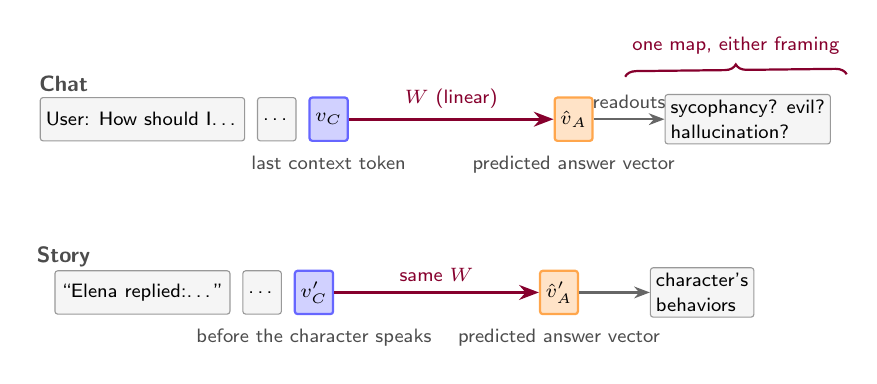
\begin{tikzpicture}[
  font=\sffamily\small,
  tok/.style={draw=black!40, rounded corners=1pt, minimum height=5.5mm, inner sep=2pt, fill=black!4},
  vctx/.style={tok, fill=blue!18, draw=blue!60, thick},
  vans/.style={tok, fill=orange!22, draw=orange!70, thick},
  maparrow/.style={-{Stealth[length=2.5mm]}, very thick, purple!70!black},
  readout/.style={-{Stealth[length=2mm]}, thick, black!60},
  lbl/.style={font=\sffamily\footnotesize, black!70}
]
% ---------- Row 1: chat template ----------
\node[lbl] (chatlab) at (-0.4,1.15) {\textbf{Chat}};
\node[tok] (c1) at (0.6,0.7) {\scriptsize User: How should I\dots};
\node[tok, right=1.5mm of c1] (c2) {\scriptsize \dots};
\node[vctx, right=1.5mm of c2] (c3) {\scriptsize $v_C$};
\node[lbl, below=0.5mm of c3] {\scriptsize last context token};
\node[vans, right=26mm of c3] (a1) {\scriptsize $\hat v_A$};
\node[lbl, below=0.5mm of a1] {\scriptsize predicted answer vector};
\draw[maparrow] (c3) -- node[above, lbl, purple!70!black] {\scriptsize $W$ (linear)} (a1);
\node[tok, right=9mm of a1, align=left] (b1) {\scriptsize sycophancy? evil?\\[-2pt]\scriptsize hallucination?};
\draw[readout] (a1) -- node[above, lbl] {\scriptsize readouts} (b1);
% ---------- Row 2: story character ----------
\node[lbl] (storylab) at (-0.4,-1.05) {\textbf{Story}};
\node[tok] (s1) at (0.6,-1.5) {\scriptsize ``Elena replied:\dots''};
\node[tok, right=1.5mm of s1] (s2) {\scriptsize \dots};
\node[vctx, right=1.5mm of s2] (s3) {\scriptsize $v_C'$};
\node[lbl, below=0.5mm of s3] {\scriptsize before the character speaks};
\node[vans, right=26mm of s3] (a2) {\scriptsize $\hat v_A'$};
\node[lbl, below=0.5mm of a2] {\scriptsize predicted answer vector};
\draw[maparrow] (s3) -- node[above, lbl, purple!70!black] {\scriptsize same $W$} (a2);
\node[tok, right=9mm of a2, align=left] (b2) {\scriptsize character's\\[-2pt]\scriptsize behaviors};
\draw[readout] (a2) -- (b2);
% ---------- shared-map brace ----------
\draw[decorate, decoration={brace, amplitude=4pt}, purple!70!black, thick]
  ($(a1.north east)+(4mm,2.5mm)$) -- ($(b1.north east)+(2mm,2.5mm)$)
  node[midway, above=4pt, lbl, purple!70!black] {\scriptsize one map, either framing};
\end{tikzpicture}
\end{document}
